%%%%%%%%%%%%%%%%%%%%%%%%%%%%%%%%%%%%%%%%%%%%%%%%%%%%%%%
%
% chapter01 - Cyber-physical Systems
%
%%%%%%%%%%%%%%%%%%%%%%%%%%%%%%%%%%%%%%%%%%%%%%%%%%%%%%%

%
% >>>>>>>>>>>>>>> PLEASE NOTE <<<<<<<<<<<<<<<
%
% This file is not stand-alone compileable as it is, to make it compileable while writing uncomment the preamble below.
% In this case, you also have to uncomment the begin/end document statements.
% You can outcomment the preamble and the begin/end document statements again or erase them when handing in your contribution.
%
% If you use BibTex for your bibliography, please use \putbib[bibliography] to print your reference (see end of this file).
%
% you can use paths relative to your chapter dir, e.g. \figure{assets/fig1}.
%
% >>>>>>>>>>>>>>>>>>>><<<<<<<<<<<<<<<<<<<<<<<

%%%%%%%%%%%%%%%%%%%%%%%%%%%%%%%%%%%%%%%%%%%%%%%%%%
%% you can uncomment the following preamble during development to make this file compileable.
%% Note that you need the svmult.cs file inside your chapter root dir to make this work.
%% Also note that if you need additional packages etc., you can add them here, but please
%% mark them somehow so the editor of this book knows you need them in the final book.
%% When you hand in your contribution, please uncomment or remove the preamble again.
%%%%%%%%%%%%%%%%%%%%%%%%%%%%%%%%%%%%%%%%%%%%%%%%%%
%%%%%%%%%%%%%%%%%%%%%%%%%%%%%%%%%%%%%%%%%%%%%%%%%%% start of preamble
%\documentclass[
%graybox,
%envcountchap,
%natbib
%]{svmult}
\documentclass[
graybox,
envcountchap
]{svmult}

\usepackage[utf8]{inputenc}
\usepackage{type1cm}        % activate if the above 3 fonts are not available on your system

\usepackage{makeidx}         % allows index generation
\usepackage{graphicx}        % standard LaTeX graphics tool when including figure files
\usepackage{multicol}        % used for the two-column index
\usepackage[bottom]{footmisc}% places footnotes at page bottom

\usepackage{newtxtext}       % 
\usepackage{newtxmath}       % selects Times Roman as basic font

\usepackage{footmisc}

% Additional packages added. Add necessary packages here.
\usepackage[english]{babel}
\usepackage{siunitx}
\usepackage{amssymb}
\usepackage{pifont}
\usepackage{xcolor}
\usepackage{tabularx}
\usepackage{listings}
\usepackage{booktabs}
\usepackage{hyperref}
\usepackage{url}
\usepackage{mathtools}
\usepackage{lipsum}
\usepackage{import}
\usepackage{bibunits}
\usepackage{acronym}
\usepackage[nottoc]{tocbibind}
%\usepackage{numberpt}
\usepackage{todonotes}


\usepackage{tikz}
\usepackage{color}
\usetikzlibrary{calc,shapes,automata,backgrounds,petri}
\tikzstyle{haState}=[rectangle split,rectangle split parts=2,draw,align=center,rounded corners]


\newcommand*{\CHAPTERSROOT}{../.}	% root path for chapters.
\newcommand*{\chapterprefix}{01}	% your chapter number.

\makeindex % used for the subject index
%%end of preamble

%uncomment the \begin{document} statement to make this file stand-alone compileable.
\begin{document}

\begin{bibunit}
	
\title*{Cyber-physical Systems}
\author{Carlos Varela and Damien Zufferey}
	
\institute{
	Carlos Varela \at Rensselaer Polytechnic Institute, USA, \email{cvarela@cs.rpi.edu}
	\and Damien Zufferey \at Max Planck Institute for Software Systems, Germany, \email{zufferey@mpi-sws.org}
	\and Gul Agha \at University of Illinois, USA, \email{agha@illinois.edu}
	\and Takuo Watanabe \at Tokyo Institute of Technology, Japan, \email{takuo@c.titech.ac.jp}
	\and Shoji Yuen \at Nagoya University, Japan, \email{yuen@is.nagoya-u.ac.jp}
	\and Marjan Sirjani \at Mälardalen University, Sweden, \email{marjan.sirjani@mdh.se}
	\and YoungMin Kwon \at SUNY Stonybrook, Korea, \email{youngmin.kwon@sunykorea.ac.kr}
}
\maketitle
	
\abstract{Please place your abstract here.}
	
%% content
%\section{Programming Cyber Physical Systems: Introduction}\label{sec:1}
\section{Motivation}\label{sec:Intro}
%(3pp)


The term Cyber-Physical Systems (CPS) broadly covers any distributed computing infrastructure interacting with the physical world in a feedback loop.
At an high level, CPS integrates communication, computation, and control.
CPS is the evolution of embedded systems as communication and distribution becomes the norm.
Development and deployment of CPS is increasing~\cite{DBLP:journals/cacm/KumarK15}.
However, CPS present their own challenges from a software perspective as the usual software abstractions are not always suitable for CPS~\cite{Lee:EECS-2008-8}.
CPS combines the challenges of normal software with the extra complexity of sensing and acting on a dynamical system.
With both distributed software and hardware components acting in a shared world, CPS can communicate explicitly through the exchange of messages and implicitly through the environment.
Communication for CPS need to account for synchronization through messages, time, and the environment.

\todo[inline]{examples: Give concrete examples of CPS and the challenges for each of them}

Consider a {\it smart wing} with piezo-electric sensors on its skin to estimate one of three conditions:  {\it normal}, {\it stall}, and {\it flutter.}  A CPS controlling the wing would need to actuate on it, e.g., reducing its angle of attack to prevent a stall or conversely, increasing its angle of attack to prevent flutter.  Structural health monitoring could also be accomplished whereby cracks detected early would restrict the flight envelope to prevent high-strain maneuvers, such as steep bank angles, that would impose prohibitive loads on damaged areas.

Consider a {\it smart building} with temperature and humidity sensors and actuators that aims to maximize occupants' comfort while minimizing energy consumption.  \todo{Please add some desired properties here.}

Consider a {\it smart car} with multiple cameras, LIDAR, sound, and multimodal sensors navigating in an open environment.  A CPS controlling the car would need to accelerate, slow down, or stop the vehicle if a collision is imminent.

All these {\it smart infrastructure} scenarios depend on sensors providing accurate information and actuators working reliably.  When sensors or actuators fail, it is critical to have both physical and analytical redundancy to detect and isolate the failure, reconfigure the CPS system, and model its behavior under such failure to enable reasoning about its dynamic behavior.

In this chapter, we will describe modeling and reasoning techniques, programming and verification methodologies, and algorithmic and communication aspects for CPS.  We will conclude by discussing open research questions to address the challenges of future CPS.

\section{Modeling and Reasoning} %(3pp)

Many computational approaches have been developed for concurrent and real-time communication and computation, but few cover the combination of communication, and dynamic control of physical state.
In this section, we give a short overview of models used to formalize CPS.

     \subsection{Temporal logics}
     
    \subsection{Control theory}

Control theory approach (plant model and feedback controller), discuss the kind of property like stability

    \subsection{Hybrid and Timed Automata}

Modeling paradigms for hybrid systems such as hybrid automata and its extensions \cite{DBLP:conf/lics/Henzinger96,AlurGLS06,DBLP:journals/iandc/LynchSV03} allow expressive dynamics, but little support for compositional programming and reasoning about communication.
Hybrid Automaton extends discrete state-based models, i.e. automata, with the continuous evolution of a dynamical systems.
Each state of an hybrid automaton is associated with a set of ordinary differential equations (ODE) and an invariant.
The transitions are guarded with expressions ranging over the continuous variables.
Fig.~\ref{fig:HA-ex1} shows an hybrid automaton.

\begin{figure}
\centering
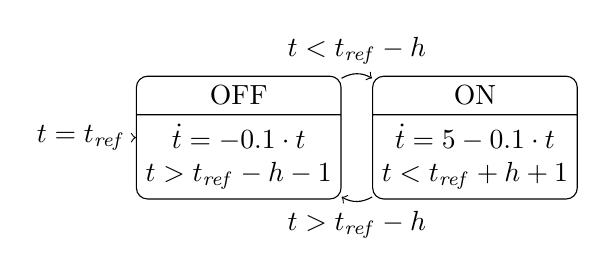
\begin{tikzpicture}[->, auto, node distance=2cm]

    \node[haState] (off) { OFF \nodepart{second} $\dot t = -0.1 \cdot t$ \\ $t > t_{\mathit{ref}} - h - 1$ };
    \node[haState] (on) [right of=off,xshift=1cm] { ON  \nodepart{second} $\dot t = 5 -0.1 \cdot t$ \\ $t < t_{\mathit{ref}} + h + 1$ };
    \node (init) [left of=off] {$t = t_{\mathit{ref}}$};

    \path (init) edge (off);
    \path (off) edge [bend left] node[above] { $t < t_{\mathit{ref}} - h$ } (on);
    \path (on) edge [bend left] node[below] { $t > t_{\mathit{ref}} - h$ } (off);

\end{tikzpicture}

% t is current temp
% t_ref is target temp
% h is hysteresis
\caption{Hybrid automata representing a bang-bang controller for an heating system.}
\label{fig:HA-ex1}
\end{figure}

An run of an hybrid automaton is an sequence of discrete \emph{jumps} and continuous \emph{flows}.
When the automaton is in a state, the continuous state changes, or flows, as described by the state's ODE.
A discrete jumps can happen when the guard of the corresponding transition evaluates to true.
A jump does two changes to the automaton: (1) it changes the automaton's state and (2) it can changes the values of the continuous states.

Hybrid automaton does not natively include any mechanism for communication.
Communication needs to be encoded within the finite state structure of the automaton.

For the most part, analysis algorithms for these models are intractable.
Timed automata~\cite{DBLP:journals/tcs/AlurD94} are a special case of hybrid automata where all the continuous dimension are clocks which increase at constant speed.
The guards on the transitions are limited to difference logic, i.e. inequalities with at most two clock variables.
This model is expressive enough to express real-time constraints and can by analyzed efficiently. %emptiness is PSpace

% Should we also discuss communicating state machines along with automata

    \subsection{Process Algebra and Differential Dynamic Logic}

Hybrid process algebras \cite{RoundsS03,BERGSTRA2005215,10.1007/978-3-319-53733-7_8,DBLP:conf/case/CampbellTLPOF16} and Differential dynamic logic \cite{PlatzerBook,Platzer18,PlatzerT18} has been developed for the deductive verification for hybrid systems attempts to define logics and invariant-based reasoning to hybrid systems.
These models enable reasoning about arbitrarily complex concurrent and hybrid programs.
Differential dynamic logic is a general logical framework to deductively reason about hybrid systems.
It extends dynamic logic with differential operators and shows sound and (relatively) complete axiomatizations for the logic.
Keymaera \cite{QueselMLAP16} is an interactive theorem prover based on this approach and it has been used to successfully verify some complex models.
Extensions of differential dynamic logic have been used to model loosely coupled distributed hybrid systems \cite{Platzer12}.
However, it has not been extended with structured message-based concurrency or with resource reasoning.

% DZ: restructure
% 1. process algebra, take the \phi-calculus as an example
% 2. session types with time and motion
% 3. DDL
\todo[inline]{explain what it is and give an example}

    \subsection{Markov Processes}

Concurrent systems are often modeled by a state transition system, such as Kripke structure, where uncertainties in the state transitions are captured by nondeterministic choices of the next state. Properties of such systems can be described using temporal logics such as LTL, CTL, and CTL*. Through a computerized process called model checking, a model can be validated against such properties.

Replacing the nondeterminism in the state transition with state transition probabilities, the state transition systems can be modeled by Markov chains. A Continuous Time Markov Chain (CTMC) comprises a set of states and an infinitesimal generator matrix, representing the rate of the state transition between two states. Similarly, a Discrete Time Markov Chain (DTMC) comprises a set of states and a probability transition matrix, representing the probability of the state transition between two states. Temporal logics like PCTL and PCTL* and their model checkers have been used to quantitatively describe and validate the probability of satisfying certain properties of a model.

Another research direction on Markov chains is to describe statistical properties of a large scale system. In this approach, the state of a system as a whole is a Probability Mass Function (PMF), representing the portions of individual systems in a certain state and the computation paths are the trajectories of PMFs over time. iLTL is a probabilistic temporal logic that can describe the evolutions of PMFs from their initial states to limiting states. 

\begin{figure}
\centering
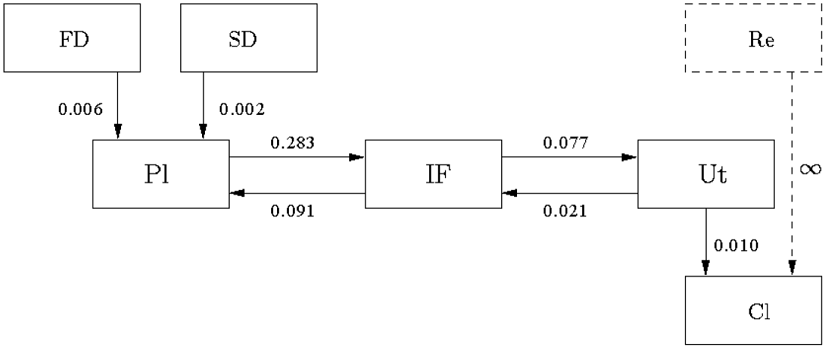
\includegraphics[width=.6\columnwidth]{assets/compartment_model.png}
\caption{
    A compartment model (CTMC), describing a drug ADME process: the boxes are the compartments representing Fast-acting Drug, Slow-acting Drug, Plasma, Interstitial Fluid, Site of Utilization, and Cleared respectively; and the numbers are the state transition rates. Re is an artificial state, where the drug is cleared instantly.}
\label{fig:comparment}
\end{figure}

For example, Fig.~\ref{fig:comparment} shows a compartment model for a drug Absorption, Distribution, Metabolism, and Excretion (ADME) process. Compartment models are a Markov chain that has been used in Pharmaceutics to describe drug kinetics. Using iLTL one can specify desirable properties such as a minimum toxic concentration, minimum effective concentration, conditions for multi-dosage regimen, etc. and find a prescription (the portions of drug in FD, SD, and Re at the initial state) that can satisfy the specification.


\subsection{Actor Models and Timed Rebeca??}
%\subsection{Actor Model}
The Reactive Object Language, Rebeca, is an actor-based modeling language  supported by a model checking tool Afra.
Rebeca is used for modeling and formal verification of concurrent and distributed systems that are mainly event-driven and asynchronous.


\subsection{Functional Reactive Programming}

    communication using streams
    
\section{Programming and Verification}\label{sec:Programming}

Starting from more general-purpose languages, like Erlang, ABCL, and Salsa ...

Talk about fairness problems ... these languages are designed for distributed systems.

If we consider CPS covering different dimensions: distributed systems, real-time, hybrid (interface of physical and cyber), then we can talk about languages addressing "distributed" systems,  "real-time" systems.

Then talk about the domain specific languages that target CPS.

Like Pilot and Lingua Franca
%DZ: maybe discuss ROS, not really a language but based around message passing and communication

\subsection{Lingua Franca}
Actor-based, a coordination language for cyber-physical systems

\section{Communication} %(4pp)

CPS need communication at the level of the controllers to achieve some goals.
At the physical level, the physical elements of a CPS influence with each other and the controllers need to adapt.
Communication between processes is the main mechanism, at the controller level, used when one process observations or actuation capabilities are insufficient to allow it to satisfies its specification independently.
In Fig.~\ref{fig:HA-ex2}, we show an extension of the example from Fig.~\ref{fig:HA-ex1} with two adjacent rooms each having its own heating system.
We highlight in {\color{red!90!black}red} the interaction of the two physical elements.
As the room are adjacent, heats spread between the two.
As presented, this system does not use communication.
However, we could imagine that there are constraint on the power for the system and that it is not possible to have both heating ON at the same time, i.e.~the lower right state does not exist.
In that case, coordination between the two controller is required.


\begin{figure}
\centering
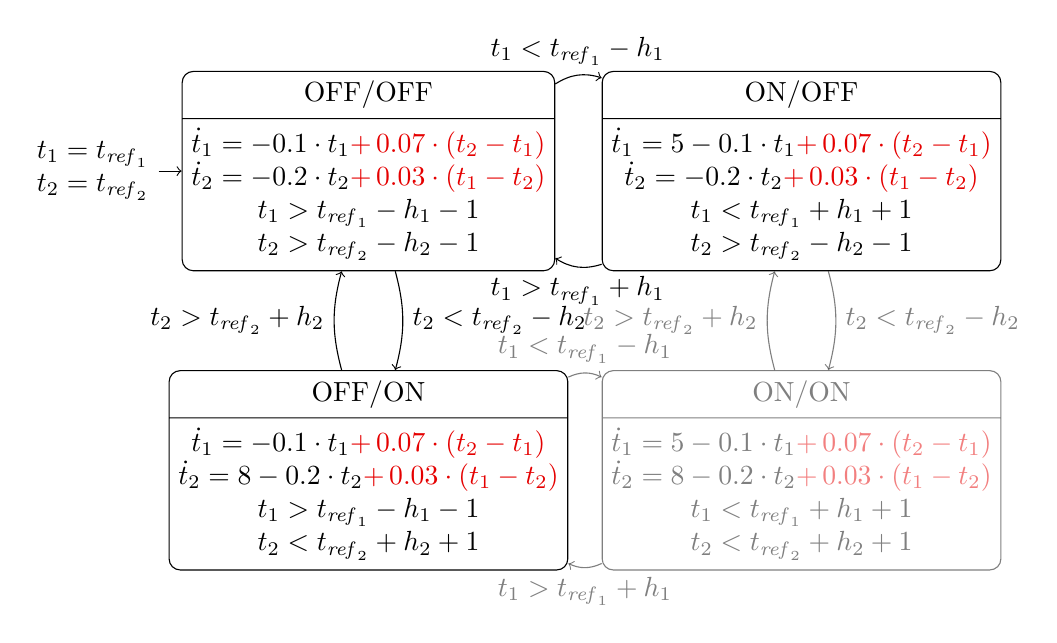
\begin{tikzpicture}[->, auto, node distance=45mm]

    \node[haState] (offoff) {
        OFF/OFF \nodepart{second}
        $\dot t_1 = -0.1 \cdot t_1 \color{red!90!black}{ +\, 0.07 \cdot (t_2 - t_1)}$ \\
        $\dot t_2 = -0.2 \cdot t_2 \color{red!90!black}{ +\, 0.03 \cdot (t_1 - t_2)}$ \\
        $t_1 > t_{\mathit{ref}_1} - h_1 - 1$ \\
        $t_2 > t_{\mathit{ref}_2} - h_2 - 1$
    };
    \node[haState] (onoff) [right of=offoff,xshift=1cm] {
        ON/OFF \nodepart{second}
        $\dot t_1 = 5 -0.1 \cdot t_1 \color{red!90!black}{ +\, 0.07 \cdot (t_2 - t_1)}$ \\
        $\dot t_2 =   -0.2 \cdot t_2 \color{red!90!black}{ +\, 0.03 \cdot (t_1 - t_2)}$ \\
        $t_1 < t_{\mathit{ref}_1} + h_1 + 1$ \\
        $t_2 > t_{\mathit{ref}_2} - h_2 - 1$
    };
    \node[haState] (offon) [below of=offoff,yshift=7mm] {
        OFF/ON \nodepart{second}
        $\dot t_1 =   -0.1 \cdot t_1 \color{red!90!black}{ +\, 0.07 \cdot (t_2 - t_1)}$ \\
        $\dot t_2 = 8 -0.2 \cdot t_2 \color{red!90!black}{ +\, 0.03 \cdot (t_1 - t_2)}$ \\
        $t_1 > t_{\mathit{ref}_1} - h_1 - 1$ \\
        $t_2 < t_{\mathit{ref}_2} + h_2 + 1$
    };
    \node[haState,semitransparent] (onon) [below of=onoff,yshift=7mm] {
        ON/ON  \nodepart{second}
        $\dot t_1 = 5 -0.1 \cdot t_1 \color{red!90!black}{ +\, 0.07 \cdot (t_2 - t_1)}$ \\
        $\dot t_2 = 8 -0.2 \cdot t_2 \color{red!90!black}{ +\, 0.03 \cdot (t_1 - t_2)}$ \\
        $t_1 < t_{\mathit{ref}_1} + h_1 + 1$ \\
        $t_2 < t_{\mathit{ref}_2} + h_2 + 1$
    };
    \node[align=center] (init) [left of=offoff,xshift=1cm] {
        $t_1 = t_{\mathit{ref}_1}$ \\
        $t_2 = t_{\mathit{ref}_2}$
    };

    \path (init) edge (offoff);
    \path (offoff) edge [bend left=25]  node[above] { $t_1 < t_{\mathit{ref}_1} - h_1$ } (onoff);
    \path (onoff)  edge [bend left=25]  node[below] { $t_1 > t_{\mathit{ref}_1} + h_1$ } (offoff);
    \path (offoff) edge [bend left=15]  node[right] { $t_2 < t_{\mathit{ref}_2} - h_2$ } (offon);
    \path (offon)  edge [bend left=15]  node[left]  { $t_2 > t_{\mathit{ref}_2} + h_2$ } (offoff);
    \path[semitransparent] (offon)  edge [bend left=25]  node[above] { $t_1 < t_{\mathit{ref}_1} - h_1$ } (onon);
    \path[semitransparent] (onon)   edge [bend left=25]  node[below] { $t_1 > t_{\mathit{ref}_1} + h_1$ } (offon);
    \path[semitransparent] (onoff)  edge [bend left=15]  node[right] { $t_2 < t_{\mathit{ref}_2} - h_2$ } (onon);
    \path[semitransparent] (onon)   edge [bend left=15]  node[left]  { $t_2 > t_{\mathit{ref}_2} + h_2$ } (onoff);

\end{tikzpicture}

\caption{
    Hybrid automata representing a the product of two bang-bang controllers for an heating system.
}
\label{fig:HA-ex2}
\end{figure}

In the previous section, we introduced a models for CPS.
Now, we looks at the role and influence of communication models.

    \subsection{Synchronous rendez-vous communication}

Synchronous communication is arguably the simplest communication model.
It is easy to define, e.g. $P \stackrel{!a}{\rightarrow} P' \land Q \stackrel{?a}{\rightarrow} Q' \Rightarrow P \mid Q \stackrel{\tau}{\rightarrow} P' \mid Q'$.
As it does not increase the state-space, i.e.~no channels as extra memory, it is also the easiest to analyze.

For CPS, synchronous communication is suitable for system's where the systems dynamic is slow w.r.t. the message propagation delay.
However, synchronous communication has some drawback.
It this model, processes block both on sending and receiving.
Most message-passing implementation only blocks on receiving.
Therefore, is is often used in conjunction with extra sufficient conditions to prevent blocking.
For instance, a process is required to be ready to receive a messages at any time \cite{?}. \todo{find ref (interface automata ?)}



    \subsection{Networked Control System}

    centralized vs distributed controller

\section{Algorithmic and Implementation Aspects} %(2pp)

    Similar to consistency question in distributed system, the freshness of physical information is important for CPS.
    The main difference between data consistency for CPS and non-CPS is that instead of a logical of operations, CPS are sensitive to time.
    In previous section, we discussed general models which model time and communication in various ways.
    In this section, we review general strategies which can be used to deal with time and communication assuming that continuous time and communication with bounded delay, i.e., there is a lower and upper bound on the time it takes to send a message.

    \subsection{Clock Synchronization}
    
    As processes share the same physical world which implicitly assume the existence of a global time.
    At the software level, clock synchronization protocols are used to establish a common time shared by all the processes.
    Clock synchronization forms the basis on which other functionalities are built.
    For instance, a common strategy in control is to build a model of the system which can be used for prediction and the optimize what the controller does (Model Predictive Control).
    In the case of CPS, estimating the state of the system requires exchanging messages and, because of the communication delay, processes need to add timestamps to the sensor reading sent over messages.
    With this information, it is possible to build an coherent model of the system.
    While synchronized clocks are most of the time assumed and used at the application level, it is also possible to rely on it while the semantics of programming language \cite{DBLP:conf/dac/LohstrohSGWGSL19,DBLP:conf/emsoft/LohstrohSJWL19}.
    
    The most commonly used clock synchronization protocols are Network Time Protocol (NTP) \cite{rfc5905} and Precision Time Protocol (PTP) \cite{4579760}.
    Both these protocol works by periodically sending timestamped messages to estimate and correct the time difference between a reference time source and the local clock.
    NTP is implemented purely in software and can achieve millisecond accuracy and PTP, with hardware support, can achieve microsecond accuracy.
    A more in depth overview of this field is found in a survey by L\'evesque and Tipper \cite{DBLP:journals/comsur/LevesqueT16}.
  
    \subsection{State Estimation, Interpolation, and Extrapolation}
    
    Wider discussion about state estimation: (extended) Kalman filter, particle filter, etc.
    This can then used for interpolation and extrapolation.
    Example: ROS uses timestamp all over the place, e.g. the TF2 library use timestamped messages to interpolate/extrapolate data    
   
    \subsection{Robustness against Perturbation of Communication}

    example: work on Skorokhod Distance by Rupak Majumdar \cite{DBLP:conf/cav/DeshmukhMP15,DBLP:conf/hybrid/MajumdarP15} and similar work by Ichiro Hasuo \cite{DBLP:conf/cyphy/KidoSH17,DBLP:conf/adhs/KidoSH18}



    \subsection{Efficient Use of Communication}

    Simple strategy: devise a centralised controller and have processes send messages to each other so that they can each have a sufficiently complete view of the global system.
    Then each process can compute what it needs to do using the central model and act accordingly.
    The time-triggered approach fixes a time interval small enough for the controller to work.
    However, this can be quite inefficient as the communication only depends on time and not on what the underlying physical system does.
    A different strategy is event-triggered control.
    The starting point is similar, each process maintains a copy of the global model.
    When it detects a significant deviation between what it locally measure and the model, then it sends messages to the other processes so they can update their model.
    This can lead to more efficient use of the network.
    When the system evolve slowly and the disturbances are small, little communication is needed.
    When the disturbance are larger and the systems has a faster dynamic, more messages are exchanged.
    Example: work by Sebastian Trimpe on event triggered and wireless control systems



\section{Open Research Questions} %(2-5pp)

    \subsection{Discrete and continuous systems}

    Process algebra, actors, and others model discrete systems.
    Differential equations, calculus, and others model the physical world.

    \begin{itemize}
    \item How to incorporate continuous time and space into concurrency models?
    \item How to go beyond bi-simulation and observational equivalence to reason about continuous systems?
    \end{itemize}
    
    \subsection{Hardware/Software interface}

    Cyber-physical systems have a hardware (physical) and a software (cyber) component
    
    \begin{itemize}
    \item How to model SW/HW interface?
    \item Are real-time properties properly modeled?
    \item  How to tackle complexity via abstraction without losing key properties?  (Translucency vs black box approaches)
    \item How to verify infinite-space systems?
    \end{itemize}

    \subsection{Dealing with uncertainty}

    Stochastic nature of cyber-physical systems, e.g., weather, requires probabilistic approach.
    
    \begin{itemize}
    \item Are heterogeneous latencies, failure modes properly accounted for?
    \item How to accurately model, quantify, propagate uncertainty?
    \item Need for statistical reasoning libraries suitable for interactive/automated proof assistants.
    \end{itemize}

    \subsection{Modal logics and reasoning}
    
    \begin{itemize}
    \item  Is first-order logic sufficient to reason about cyber-physical systems?
    \item Are spatial logics, temporal logics, and combinations thereof better suited for specifying and reasoning about CPS?
    \item What are their expressive power?   Are there efficient decision procedures?  (SAT modulo theory approaches?)
    \end{itemize}

    \subsection{Robust control}

    Can we reason about properties of feedback loop control systems incorporating the above (hybrid, SW/HW/Network, uncertainty/failures, modal logics/reasoning)?
    
    \subsection{AI and data-driven systems}

    As more CPS are model-driven and more models are data-driven, how can we trust these systems?  Are there inherent theoretical limits to dynamic data-driven applications and systems? (e.g., Cramer-Rao lower bounds, etc.)

	% \section*{Appendix}\label{appendix}
	
	% Please place your appendix content here, if applicable.
	
	%%%%%%%%%%%%%%%%%%%%%%%%%%%%%%%%%%%%%%%%%%%%%%%%%%%%%%%%%%%%%%%%%%%%%%%%%%%%%%%%%%%%%%%%%%%%%%%%%%%%%%%%
	%% For your bibliography, you should use a bibtex .bib file and include it here.
	%% Note that the final reference lists styling might differ because it'll be styled in unified book layout.
	
	% \biblstarthook{
	%	text inserted here will be printed before the actual list of references, but only if there is at least one reference to %display. Delete this section if you don't need it.
	%}
	
	% \nocite{*}		%% uncomment if uncited references should be listed in the bibliography.
	
	%% uncomment and state path to your .bib to use a bibtex file as your bibliography.
	%% NOTE: relative paths don't work in \putbib => During development, you might delete the "\CHAPTERSROOT/chapter\chapterprefix/" part to refer to your bib file. When you're done, please make this path absolute by adding the prefix again.
	%%
    \putbib[\CHAPTERSROOT/chapter\chapterprefix/bibliography] %
	%\putbib[bibliography] %
	
\end{bibunit}
	
%% uncomment the \end{document} statement to make this file stand-alone compileable.
\end{document}
